\documentclass[10pt]{article}
\usepackage[utf8]{inputenc}
\usepackage[T1]{fontenc}
\usepackage{amsmath}
\usepackage{amsfonts}
\usepackage{amssymb}
\usepackage{mhchem}
\usepackage{stmaryrd}
\usepackage{graphicx}
\usepackage[export]{adjustbox}
\graphicspath{ {./images/} }
\usepackage{bbold}

\title{Probability and training algorithms }

\author{}
\date{}


\begin{document}
\maketitle
\section{Contents}
$1 \quad$ Probability and training algorithms $\ldots \ldots \ldots \ldots \ldots \ldots \ldots \ldots \ldots \ldots . \ldots$

$1.1$ Convex functions and convergence of gradient descent $\ldots \ldots \ldots \ldots .3$

1.1.1 Convex function $\ldots \ldots \ldots \ldots \ldots \ldots \ldots \ldots . \ldots \ldots \ldots$

$1.1 .2$ On the Convergence of GD $\ldots \ldots \ldots \ldots \ldots \ldots \ldots \ldots \ldots \ldots \ldots \ldots \ldots \ldots \ldots \ldots \ldots \ldots \ldots$


\includegraphics[max width=\textwidth]{2022_03_25_9faca01b68c57c6da639g-2}

\subsection{Convex functions and convergence of gradient descent}
\subsubsection{Convex function}
Then, let us first give the definition of convex sets.

Definition 1 (Convex set). A set $C$ is convex, if the line segment between any two points in $C$ lies in $C$, i.e., if any $x, y \in C$ and any $\alpha$ with $0 \leq \alpha \leq 1$, there holds
$$
\alpha x+(1-\alpha) y \in C
$$
Here are two diagrams for this definition about convex and non-convex sets.\\

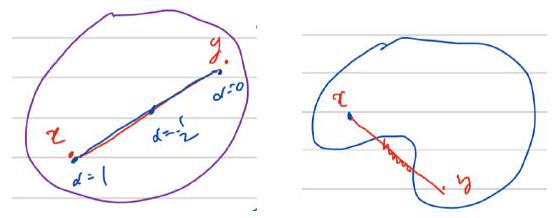
\includegraphics[max width=\textwidth]{2022_03_25_9faca01b68c57c6da639g-3}

Following the definition of convex set, we define convex function as following.

Definition 2 (Convex function). Let $C \subset \mathbb{R}^{n}$ be a convex set and $f: C \rightarrow \mathbb{R}$ :

\begin{enumerate}
  \item $f$ is called convex if for any $x, y \in C$ and $\alpha \in[0,1]$
\end{enumerate}
$$
f(\alpha x+(1-\alpha) y) \leq \alpha f(x)+(1-\alpha) f(y) .
$$

\begin{enumerate}
  \setcounter{enumi}{2}
  \item $f$ is called strictly convex if for any $x \neq y \in C$ and $\alpha \in(0,1)$ :
\end{enumerate}
$$
f(\alpha x+(1-\alpha) y)<\alpha f(x)+(1-\alpha) f(y) .
$$
1.1. CONVEX FUNCTIONS AND CONVERGENCE OF GRADIENT

DESCENT Jinchao Xu

\begin{enumerate}
  \setcounter{enumi}{3}
  \item A function $f$ is said to be (strictly) concave if $-f$ is (strictly) convex.
\end{enumerate}
We also have the next diagram for convex function definition.

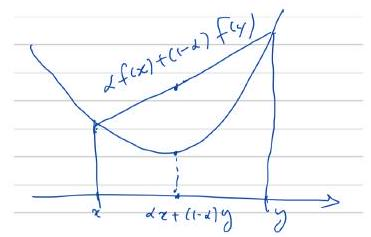
\includegraphics[max width=\textwidth]{2022_03_25_9faca01b68c57c6da639g-4}

Lemma 1. If $f(x)$ is differentiable on $\mathbb{R}^{n}$, then $f(x)$ is convex if and only if
$$
f(x) \geq f(y)+\nabla f(y) \cdot(x-y), \forall x, y \in \mathbb{R}^{n} .
$$
Based on the lemma, we can first have the next new diagram for convex functions.

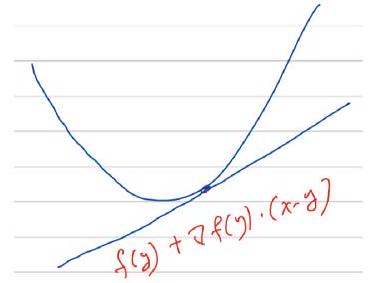
\includegraphics[max width=\textwidth]{2022_03_25_9faca01b68c57c6da639g-4(1)}

Proof. Let $z=\alpha x+(1-\alpha) y, 0 \leq \alpha \leq 1, \forall x, y \in \mathbb{R}^{n}$, we have these next two Taylor expansion:
$$
\begin{aligned}
&f(x) \geq f(z)+\nabla f(z)(x-z) \\
&f(y) \geq f(z)+\nabla f(z)(y-z)
\end{aligned}
$$
Then we have
$$
\begin{aligned}
& \alpha f(x)+(1-\alpha) f(y) \\
\geq & f(z)+\nabla f(z)[\alpha(x-z)+(1-\alpha)(y-z)] \\
=& f(z) \\
=& f(\alpha x+(1-\alpha) y) .
\end{aligned}
$$
Thus we have
$$
\alpha f(x)+(1-\alpha) f(y) \geq f(\alpha x+(1-\alpha) y)
$$
This finishes the proof.

On the other hand (homework): if $f(x)$ is differentiable on $\mathbb{R}^{n}$, then $f(x) \geq f(y)+$ $\nabla f(y) \cdot(x-y), \forall x, y \in \mathbb{R}^{n}$ if $f(x)$ is convex.

Definition 3 ( $\lambda$-strongly convex). We say that $f(x)$ is $\lambda$-strongly convex if
$$
f(x) \geq f(y)+\nabla f(y) \cdot(x-y)+\frac{\lambda}{2}\|x-y\|^{2}, \quad \forall x, y \in C,
$$
for some $\lambda>0$.

Example 1. Consider $f(x)=\|x\|^{2}$, then we have
$$
\frac{\partial f}{\partial x_{i}}=2 x_{i}, \nabla f=2 x \in R^{n}
$$
So, we have
$$
\begin{aligned}
& f(x)-f(y)-\nabla f(y)(x-y) \\
=&\|x\|^{2}-\|y\|^{2}-2 y(x-y) \\
=&\|x\|^{2}-\|y\|^{2}-2 x y+2\|y\|^{2} \\
=&\|x\|^{2}-2 x y+\|y\|^{2} \\
=&\|x-y\|^{2} \\
=& \lambda\|x-y\|^{2}, \quad \lambda=2 .
\end{aligned}
$$
Thus, $f(x)=\|x\|^{2}$ is 2-strongly convex

Example 2 (Homework). Actually, the loss function of the logistic regression model
$$
L(\theta)=-\log P(\theta)
$$
is convex as a function of $\theta$.

Furthermore, the loss function of the regularized logistic regression model
$$
L_{\lambda}(\theta)=-\log P(\theta)+\lambda\|\theta\|_{F}^{2}, \lambda>0
$$
is $\lambda^{\prime}$-strongly convex $\left(\lambda^{\prime}\right.$ is related to $\left.\lambda\right)$ as a function of $\theta$.

We also have these following interesting properties of convex function.

Properties 1 (basic properties of convex function) [Homework]

\begin{enumerate}
  \item If $f(x), g(x)$ are both convex, then $\alpha f(x)+\beta g(x)$ is also convex, if $\alpha, \beta \geq 0$. 1.1. CONVEX FUNCTIONS AND CONVERGENCE OF GRADIENT
\end{enumerate}
$\frac{\text { DESCENT }}{\text { 2. Linear function is both convex and concave. Here, } f(x) \text { is concave if and only if }}$ - Linear function is

\begin{enumerate}
  \setcounter{enumi}{3}
  \item If $f(x)$ is a convex convex function on $\mathbb{R}^{n}$, then $g(y)=f(A y+b)$ is a convex function on $\mathbb{R}^{m}$. Here $A \in \mathbb{R}^{m \times n}$ and $b \in \mathbb{R}^{m}$.

  \item If $g(x)$ is a convex function on $\mathbb{R}^{n}$, and the function $f(u)$ is convex function on $\mathbb{R}$ and non-decreasing, then the composite function $f \circ g(x)=f(g(x))$ is convex.

\end{enumerate}
Proof. Homework: prove them by definition.

\subsubsection{On the Convergence of GD}
For the next optimization problem
$$
\min _{x \in \mathbb{R}^{n}} f(x)
$$
We assume that $f(x)$ is convex. Then we say that $x^{*}$ is a minimizer if $f\left(x^{*}\right)=$ $\min _{x \in \mathbb{R}^{n}} f(x) .$

Let recall that, for minimizer $x^{*}$ we have
$$
\nabla f\left(x^{*}\right)=0
$$
Then we have the next tw properties of minimizer for convex functions:

\begin{enumerate}
  \item If $f(x) \geq c_{0}$, for some $c_{0} \in \mathbb{R}$, then we have
\end{enumerate}
$$
\arg \min f \neq \emptyset
$$

\begin{enumerate}
  \setcounter{enumi}{2}
  \item If $f(x)$ is $\lambda$-strongly convex, then $f(x)$ has a unique minimizer, namely, there exists a unique $x^{*} \in \mathbb{R}^{n}$ such that
\end{enumerate}
$$
f\left(x^{*}\right)=\min _{x \in \mathbb{R}^{n}} f(x)
$$
To investigate the convergence of gradient descent method, let recall the gradient descent method:

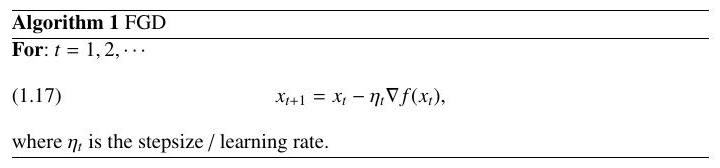
\includegraphics[max width=\textwidth]{2022_03_25_9faca01b68c57c6da639g-6}

Assumption $1.18$ We make the following assumptions 1. $f(x)$ is $\lambda$-strongly convex for some $\lambda>0$. Recall the definition, we have
$$
f(x) \geq f(y)+\nabla f(y) \cdot(x-y)+\frac{\lambda}{2}\|x-y\|^{2},
$$
then note $x^{*}=\arg \min f(x)$. Then we have

\begin{itemize}
  \item Take $y=x^{*}$, this leads to
\end{itemize}
$$
f(x) \geq f\left(x^{*}\right)+\frac{\lambda}{2}\|x-y\|^{2} .
$$

\begin{itemize}
  \item Take $x=x^{*}$, this leads to
\end{itemize}
$$
0 \geq f\left(x^{*}\right)-f(y) \geq \nabla f(y) \cdot\left(x^{*}-y\right)+\frac{\lambda}{2}\left\|x^{*}-y\right\|^{2}
$$
which means that
$$
\nabla f(x) \cdot\left(x-x^{*}\right) \geq \frac{\lambda}{2}\left\|x-x^{*}\right\|^{2}
$$

\begin{enumerate}
  \setcounter{enumi}{2}
  \item $\nabla f$ is Lipschitz for some $L>0$, i.e.,
\end{enumerate}
$$
\|\nabla f(x)-\nabla f(y)\| \leq L\|x-y\|, \forall x, y .
$$
Thus, we have the next theorem about the convergence of gradient descent method.

Theorem 2. For Algorithm 1, if $f(x)$ is $\lambda$-strongly convex and $\nabla f$ is Lipschitz for some $L>0$, then
$$
\left\|x_{t}-x^{*}\right\|^{2} \leq \alpha^{t}\left\|x_{0}-x^{*}\right\|^{2}
$$
if $0<\eta_{t} \leq \eta_{0}=\frac{\lambda}{2 L^{2}}$ and $\alpha=1-\frac{\lambda^{2}}{4 L^{2}}<1 .$

Proof. If we minus any $x \in \mathbb{R}^{n}$, we can only get:
$$
x_{t+1}-x=x_{t}-\eta_{t} \nabla f\left(x_{t}\right)-x .
$$
If we take $L^{2}$ norm for both side, we get:
$$
\left\|x_{t+1}-x\right\|^{2}=\left\|x_{t}-\eta_{t} \nabla f\left(x_{t}\right)-x\right\|^{2} .
$$
So we have the following inequality and take $x=x^{*}$ :

$(1.24)$

$\left\|x_{t+1}-x^{*}\right\|^{2}=\left\|x_{t}-\eta_{t} \nabla f\left(x_{t}\right)-x^{*}\right\|^{2}$

$=\left\|x_{t}-x^{*}\right\|^{2}-2 \eta_{t} \nabla f\left(x_{t}\right)^{\top}\left(x_{t}-x^{*}\right)+\eta_{t}^{2}\left\|\nabla f\left(x_{t}\right)-\nabla f\left(x^{*}\right)\right\|^{2}$

$\leq\left\|x_{t}-x^{*}\right\|^{2}-\eta_{t} \lambda\left\|x_{t}-x^{*}\right\|^{2}+\eta_{t}^{2} L^{2}\left\|x_{t}-x^{*}\right\|^{2} \quad(\lambda-$ strongly convex and Lipschitz $)$

$\leq\left(1-\eta_{t} \lambda+\eta_{t}^{2} L^{2}\right)\left\|x_{t}-x^{*}\right\|$.

So, if $\eta_{t} \leq \frac{\lambda}{2 L^{2}}$, then $\alpha=\left(1-\eta_{t} \lambda+\eta_{t}^{2} L^{2}\right) \leq 1-\frac{\lambda^{2}}{4 L^{2}}<1$, which finishes the proof.

Some issues on GD: 1.1. CONVEX FUNCTIONS AND CONVERGENCE OF GRADIENT

DESCENT

Jinchao Xu

\begin{itemize}
  \item $\nabla f\left(x_{t}\right)$ is very expensive to compete.

  \item GD does not yield generalization accuracy.

\end{itemize}
The stochastic gradient descent (SGD) method which we will discuss in the next section will focus on these two issues.


\end{document}